\documentclass[11pt]{article}

\usepackage{setspace}
\usepackage[letterpaper,margin=1in]{geometry}
\usepackage[parfill]{parskip}
\usepackage{graphicx}
\graphicspath{ {images/} }

\title{DES - Security Through Obscurity}
\author{Brandon Crane, Matt Frederick, Monica Singh, 
George Wood}
\date{30 September 2017}

\begin{document}
\maketitle

\thispagestyle{empty}

\section{Individual Contributions}
Team members did most of the work together. Pair programming was implemented
in the beginning to code individual modules. Matt and Monica worked together in
one pair focusing on creation and format of the individual table functions, and George and Brandon in another
focusing on file i/o, character interpretation, and program organization. These modules were then placed in
the main file accordingly. Once debugging started, it became
a whole team effort with everybody analyzing the output. To verify that our
encryption was working correctly,
George took it upon himself to run through the algorithm by hand. He worked with
a very simple key and plaintext. This process was compared to the output of the
bit strings that our program output before and after steps in the algorithm.
This processes verified that our encryption was accurate, and we were able to
continue debugging to completion as a team. Brandon drafted up the latex
document, and George created the graphs.


\section{Execution Time Graphs}

\setcounter{secnumdepth}{0}
\subsection{8 Rounds}
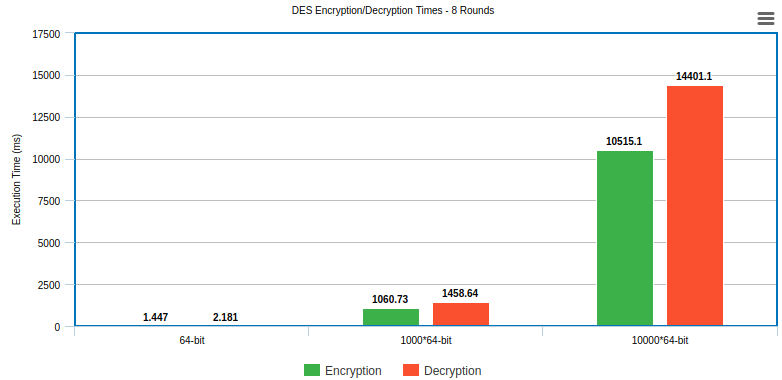
\includegraphics[scale=.8]{8RoundGraph}
\subsection{16 Rounds}
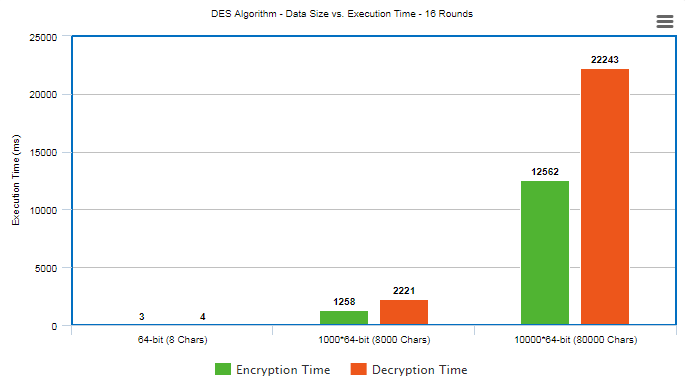
\includegraphics[scale=.8]{16RoundGraph}

\setcounter{secnumdepth}{1}
\section{Code (C++)}
\begin{verbatim}
/*
CS 455 - Project Part 1 - DES Implementation
Brandon Crane, Matt Frederick, Monica Singh, & George Wood
9/30/17
*/

#include <iostream>
#include <fstream>
#include <string>
#include <vector>
#include <bitset>
#include <time.h>
using namespace std;

//Number of characters in each block of input text being processed
const short CHARS_IN_BLOCK = 8;
//Number of bits in a char variable
const short BITS_IN_CHAR = 8;
//Number of rounds the algorithm should operate for
const short ROUND_COUNT = 8;
//Whether or not testing statements should be printed
const bool VERBOSE = false;

//IP Table, takes in vector of size 64, permutes it, and modifies
//left and right vectors passed by reference to give plaintext halves
void initPerm(vector<bool> inputVector, vector<bool>& leftText,
  vector<bool>& rightText)
{
  short outputVectorSize = 64;
  //IP table stored as an array
  short initPerm[] = {58,50,42,34,26,18,10,2,
                      60,52,44,36,28,20,12,4,
                      62,54,46,38,30,22,14,6,
                      64,56,48,40,32,24,16,8,
                      57,49,41,33,25,17,9, 1,
                      59,51,43,35,27,19,11,3,
                      61,53,45,37,29,21,13,5,
                      63,55,47,39,31,23,15,7};
  //Vector to store permuted values
  vector<bool> permVec;
  //Pushes permuted values into permVec
  for(short i=0; i < outputVectorSize; i++)
  {
    permVec.push_back(inputVector.at(initPerm[i]-1));
  }
  //First half of permuted values pushed to the leftText vector
  for (unsigned short i = 0; i < permVec.size() / 2; i++)
  {
    leftText.push_back(permVec.at(i));
  }
  //Second half of permuted values pushed to the rightText vector
  for (unsigned short i = permVec.size() / 2; i < permVec.size(); i++)
  {
    rightText.push_back(permVec.at(i));
  }
}

//Inverse IP table, takes in vector of booleans of size 64 and returns
//its permutation
vector<bool> invInitPerm(vector<bool> inputVector)
{
  short outputVectorSize = 64;
  //Inverse IP tables stored as an array
  short invInitPerm[] = {40,8,48,16,56,24,64,32,
                         39,7,47,15,55,23,63,31,
                         38,6,46,14,54,22,62,30,
                         37,5,45,13,53,21,61,29,
                         36,4,44,12,52,20,60,28,
                         35,3,43,11,51,19,59,27,
                         34,2,42,10,50,18,58,26,
                         33,1,41,9,49,17,57,25};
  //Vector of bools to be returned
  vector<bool> outputVector;
  //Pushes permuted values to outputVector
  for(short i=0; i < outputVectorSize; i++)
  {
    outputVector.push_back(inputVector.at(invInitPerm[i]-1));
  }
  return outputVector;
}

//PC1 Table, takes in vector of size 64, permutes it to size 56, and modifies
//halves passed by reference to give initial key halves
void pc1Perm(vector<bool> keyBits, vector<bool>& leftKey,
  vector<bool>& rightKey)
{
  short pcOneSize = 56;
  //PC-1 table stored as array
  short pcOne[]= {57,49,41,33,25,17,9,
                  1, 58,50,42,34,26,18,
                  10,2, 59,51,43,35,27,
                  19,11,3, 60,52,44,36,
                  63,55,47,39,31,23,15,
                  7, 62,54,46,38,30,22,
                  14,6, 61,53,45,37,29,
                  21,13,5, 28,20,12,4};
  //Pushes first half of permuted values to leftKey
  for(short i = 0; i < pcOneSize / 2; i++)
  {
    leftKey.push_back(keyBits.at(pcOne[i]-1));
  }
  //Pushes second half of permuted values to rightKey
  for(short i = pcOneSize / 2; i < pcOneSize; i++)
  {
    rightKey.push_back(keyBits.at(pcOne[i]-1));
  }
}

//Key shift scheduler, takes in key halves and shifts them by a specified
//number of bits based on the current round of encryption
vector<bool> leftShiftSched(vector<bool> inputVector, short round)
{
  //Left shift schedule stored as array
  short schedule[] = {1,1,2,2,2,2,2,2,1,2,2,2,2,2,2,1};
  //Vector of bools to be returned
  vector<bool> outputVector;
  //The following two for loops perform the left shift
  for (unsigned short i = schedule[round]; i < inputVector.size(); i++ )
  {
    outputVector.push_back(inputVector.at(i));
  }
  for(short i = 0; i < schedule[round]; i++)
  {
    outputVector.push_back(inputVector.at(i));
  }
  return outputVector;
}

//PC2 Table, takes in key halves vectors of size 28 each, permutes them,
//and returns a combined permuted key vector
vector<bool> pc2Perm(vector<bool> leftKey, vector<bool> rightKey)
{
  //Key made up of the two half keys
  vector<bool> combinedKey = leftKey;
  combinedKey.insert(combinedKey.end(), rightKey.begin(), rightKey.end());

  short pcTwoSize = 48;
  //PC-2 table stored as array
  short pcTwo[]= {14,17,11,24,1, 5, 3, 28,
                  15,6, 21,10,23,19,12,4,
                  26,8, 16,7, 27,20,13,2,
                  41,52,31,37,47,55,30,40,
                  51,45,33,48,44,49,39,56,
                  34,53,46,42,50,36,29,32};
  //Vector of bools to be returned
  vector<bool> outputVector;
  //Pushes permuted values to outputVector
  for(short i=0; i<pcTwoSize; i++)
  {
    outputVector.push_back(combinedKey.at(pcTwo[i]-1));
  }
  return outputVector;
}

//Takes in a vector of size 32, expands and permutes it with a hard-coded table,
//and returns a vector of size 48
vector<bool> eTablePerm(vector<bool> inputVector)
{
  short outputVectorSize = 48;
  //E table stored as array
  short eTable[outputVectorSize] = {32,1, 2, 3, 4, 5,
                                    4, 5, 6, 7, 8, 9,
                                    8, 9, 10,11,12,13,
                                    12,13,14,15,16,17,
                                    16,17,18,19,20,21,
                                    20,21,22,23,24,25,
                                    24,25,26,27,28,29,
                                    28,29,30,31,32,1};
  //Vector of bools to be returned
  vector<bool> outputVector;
  //Pushes permuted values to outputVector
  for (short i = 0; i < outputVectorSize; i++)
  {
    outputVector.push_back(inputVector.at(eTable[i] - 1));
  }
  return outputVector;
}

//S Boxes, takes in vector of the right half of the plaintext of size 48
//and returns a permuted and substituted vector of length 32
vector<bool> sBoxSub(vector<bool> rightTextI)
{
  //Number of groups of to be applied to the S boxes
  short bitGroupCount = 8;
  //Number of bits in each group
  short bitsInGroup = 6;
  //Vector of S boxes
  vector<vector<vector<short>>> sBoxes;
  //Temp vectors used to create S boxes
  vector<short> tempRow;
  vector<vector<short>> tempBox;

  //S Box 1
  tempRow = {14, 4, 13, 1, 2, 15, 11, 8, 3, 10, 6, 12, 5, 9, 0, 7};
  tempBox.push_back(tempRow);
  tempRow = {0, 15, 7, 4, 14, 2, 13, 1, 10, 6, 12, 11, 9, 5, 3, 8};
  tempBox.push_back(tempRow);
  tempRow = {4, 1, 14, 8, 13, 6, 2, 11, 15, 12, 9, 7, 3, 10, 5, 0};
  tempBox.push_back(tempRow);
  tempRow = {15, 12, 8, 2, 4, 9, 1, 7, 5, 11, 3, 14, 10, 0, 6, 13};
  tempBox.push_back(tempRow);
  sBoxes.push_back(tempBox);
  tempBox.clear();

  ////S Box 2
  tempRow = {15, 1, 8, 14, 6, 11, 3, 4, 9, 7, 2, 13, 12, 0, 5, 10};
  tempBox.push_back(tempRow);
  tempRow = {3, 13, 4, 7, 15, 2, 8, 14, 12, 0, 1, 10, 6, 9, 11, 5};
  tempBox.push_back(tempRow);
  tempRow = {0, 14, 7, 11, 10, 4, 13, 1, 5, 8, 12, 6, 9, 3, 2, 15};
  tempBox.push_back(tempRow);
  tempRow = {13, 8, 10, 1, 3, 15, 4, 2, 11, 6, 7, 12, 0, 5, 14, 9};
  tempBox.push_back(tempRow);
  sBoxes.push_back(tempBox);
  tempBox.clear();

  //S Box 3
  tempRow = {10, 0, 9, 14, 6, 3, 15, 5, 1, 13, 12, 7, 11, 4, 2, 8};
  tempBox.push_back(tempRow);
  tempRow = {13, 7, 0, 9, 3, 4, 6, 10, 2, 8, 5, 14, 12, 11, 15, 1};
  tempBox.push_back(tempRow);
  tempRow = {13, 6, 4, 9, 8, 15, 3, 0, 11, 1, 2, 12, 5, 10, 14, 7};
  tempBox.push_back(tempRow);
  tempRow = {1, 10, 13, 0, 6, 9, 8, 7, 4, 15, 14, 3, 11, 5, 2, 12};
  tempBox.push_back(tempRow);
  sBoxes.push_back(tempBox);
  tempBox.clear();

  //S Box 4
  tempRow = {7, 13, 14, 3, 0, 6, 9, 10, 1, 2, 8, 5, 11, 12, 4, 15};
  tempBox.push_back(tempRow);
  tempRow = {13, 8, 11, 5, 6, 15, 0, 3, 4, 7, 2, 12, 1, 10, 14, 9};
  tempBox.push_back(tempRow);
  tempRow = {10, 6, 9, 0, 12, 11, 7, 13, 15, 1, 3, 14, 5, 2, 8, 4};
  tempBox.push_back(tempRow);
  tempRow = {3, 15, 0, 6, 10, 1, 13, 8, 9, 4, 5, 11, 12, 7, 2, 14};
  tempBox.push_back(tempRow);
  sBoxes.push_back(tempBox);
  tempBox.clear();

  //S Box 5
  tempRow = {2, 12, 4, 1, 7, 10, 11, 6, 8, 5, 3, 15, 13, 0, 14, 9};
  tempBox.push_back(tempRow);
  tempRow = {14, 11, 2, 12, 4, 7, 13, 1, 5, 0, 15, 10, 3, 9, 8, 6};
  tempBox.push_back(tempRow);
  tempRow = {4, 2, 1, 11, 10, 13, 7, 8, 15, 9, 12, 5, 6, 3, 0, 14};
  tempBox.push_back(tempRow);
  tempRow = {11, 8, 12, 7, 1, 14, 2, 13, 6, 15, 0, 9, 10, 4, 5, 3};
  tempBox.push_back(tempRow);
  sBoxes.push_back(tempBox);
  tempBox.clear();

  //S Box 6
  tempRow = {12, 1, 10, 15, 9, 2, 6, 8, 0, 13, 3, 4, 14, 7, 5, 11};
  tempBox.push_back(tempRow);
  tempRow = {10, 15, 4, 2, 7, 12, 9, 5, 6, 1, 13, 14, 0, 11, 3, 8};
  tempBox.push_back(tempRow);
  tempRow = {9, 14, 15, 5, 2, 8, 12, 3, 7, 0, 4, 10, 1, 13, 11, 6};
  tempBox.push_back(tempRow);
  tempRow = {4, 3, 2, 12, 9, 5, 15, 10, 11, 14, 1, 7, 6, 0, 8, 13};
  tempBox.push_back(tempRow);
  sBoxes.push_back(tempBox);
  tempBox.clear();

  //S Box 7
  tempRow = {4, 11, 2, 14, 15, 0, 8, 13, 3, 12, 9, 7, 5, 10, 6, 1};
  tempBox.push_back(tempRow);
  tempRow = {13, 0, 11, 7, 4, 9, 1, 10, 14, 3, 5, 12, 2, 15, 8, 6};
  tempBox.push_back(tempRow);
  tempRow = {1, 4, 11, 13, 12, 3, 7, 14, 10, 15, 6, 8, 0, 5, 9, 2};
  tempBox.push_back(tempRow);
  tempRow = {6, 11, 13, 8, 1, 4, 10, 7, 9, 5, 0, 15, 14, 2, 3, 12};
  tempBox.push_back(tempRow);
  sBoxes.push_back(tempBox);
  tempBox.clear();

  //S Box 8
  tempRow = {13, 2, 8, 4, 6, 15, 11, 1, 10, 9, 3, 14, 5, 0, 12, 7};
  tempBox.push_back(tempRow);
  tempRow = {1, 15, 13, 8, 10, 3, 7, 4, 12, 5, 6, 11, 0, 14, 9, 2};
  tempBox.push_back(tempRow);
  tempRow = {7, 11, 4, 1, 9, 12, 14, 2, 0, 6, 10, 13, 15, 3, 5, 8};
  tempBox.push_back(tempRow);
  tempRow = {15, 12, 8, 2, 4, 9, 1, 7, 5, 11, 3, 14, 10, 0, 6, 13};
  tempBox.push_back(tempRow);
  sBoxes.push_back(tempBox);

  //Vector to hold
  vector<vector<bool>> bitGroups;
  //Vector of bools to be returned
  vector<bool> outputVector;
  //Loads vectors of bools into bitGroups to represent each group of bits
  for(short i=0; i < bitGroupCount; i++)
  {
    vector<bool> temp;
    for(short j = 0; j < bitsInGroup; j++)
    {
      temp.push_back(rightTextI.at((i * bitsInGroup) + j));
    }
    bitGroups.push_back(temp);
  }

  //Applies an S box to each bit group
  for(short j = 0; j < bitGroupCount; j++)
  {
    //Number of bits that will be in each group after S box application
    short outputBitCount = 4;
    //String representing row of S box to be used
    string rowString;
    //String representing column of S box to be used
    string colString;

    //Gets row value in binary
    rowString.append(bitGroups.at(j).at(0) ? "1" : "0");
    rowString.append(bitGroups.at(j).at(bitsInGroup - 1) ? "1" : "0");
    //Gets column value in binary
    for(short i = 1; i <5; i++)
    {
      colString.append(bitGroups.at(j).at(i) ? "1" : "0");
    }
    //Bitsets to convert the row and column values to decimal
    bitset<2> row (rowString);
    bitset<4> col (colString);
    //Gets the value that each bit group will be replaced with
    bitset<4> newBinary(sBoxes.at(j).at(row.to_ulong()).at(col.to_ulong()));
    //Pushes the new binary value of the current group to outputVector
    for(short i = outputBitCount - 1; i >= 0; i--)
    {
      outputVector.push_back(newBinary[i]);
    }
  }
  return outputVector;
}

//Takes in vector of size 32, permutes it using a hard-coded table,
//and returns another vector of size 32
vector<bool> pTablePerm(vector<bool> inputVector)
{
  short outputVectorSize = 32;
  //P table stored as vector
  short pTable[outputVectorSize] = {16,7, 20,21,29,12,28,17,
                                    1, 15,23,26,5, 18,31,10,
                                    2, 8, 24,14,32,27,3, 9,
                                    19,13,30,6, 22,11,4,25};
  //Vector of bools to be returned
  vector<bool> outputVector;
  //Pushes permuted values to outputVector
  for (short i = 0; i < outputVectorSize; i++)
  {
    outputVector.push_back(inputVector.at(pTable[i] - 1));
  }
  return outputVector;
}

//Prints out binary values in a vector in separated groups of 8
//(For testing purposes)
void printVector(vector<bool> inputVec)
{
  //Prints each character
  for (unsigned int i = 0; i < inputVec.size(); i++)
  {
    cout << inputVec.at(i);
    //Inserts a space between each group of 8
    if (((i + 1) % BITS_IN_CHAR == 0) && (i != 0))
    {
      cout << " ";
    }
  }
  cout << endl;
}

//Converts characters to bits and places them in a vector of bools
vector<bool> charsToBits(vector<char> inputVector)
{
  vector<bool> outputVector;
  for (short i = 0; i < CHARS_IN_BLOCK; i++)
  {
    bitset<BITS_IN_CHAR> temp(inputVector.at(i));
    for(short j = BITS_IN_CHAR - 1; j >= 0; j--)
    {
      outputVector.push_back(temp[j]);
    }
  }
  return outputVector;
}

//Converts bits to chars and appends them to a string
string bitsToChars(vector<bool> inputVector)
{
  //Output string of converted binary values to be returned
  string outputText = "";
  //Loops for each character in the block
  for (short i = 0; i < CHARS_IN_BLOCK; i++)
  {
    //String to hold the binary of the current character
    string tempString = "";
    //Adds bits for current character to string
    for (short j = 0; j < BITS_IN_CHAR; j++)
    {
      tempString += (inputVector.at((i * CHARS_IN_BLOCK) + j) ? "1" : "0");
    }
    //Puts bits in a bitset
    bitset<BITS_IN_CHAR> temp(tempString);
    //Adds converted character to the output text
    outputText += (char)temp.to_ulong();

    if (VERBOSE)
    {
      cout << "Current char:\n" << char(temp.to_ulong()) << endl;
    }
  }
  return outputText;
}

//Takes in a size 64 vector of booleans for both plaintext and the key
//and performs DES encryption on them. Returns string of ciphertext for the
//input block of plaintext
string encrypt(vector<bool> plainTextBits, vector<bool> keyBits)
{
  //Output ciphertext to be returned
  string cipherText;

  //Left half of plaintext
  vector<bool> leftTextI;
  //Right half of plainText
  vector<bool> rightTextI;
  //Left half of key
  vector<bool> leftKey;
  //Right half of key
  vector<bool> rightKey;
  //Left half of text to be used next round
  vector<bool> leftTextIPlus1;
  //Key after PC-2 table
  vector<bool> permKey;
  //Applies IP table to plaintext and splits it into halves
  initPerm(plainTextBits, leftTextI, rightTextI);
  //Applies PC-1 table to key and splits it into halves
  pc1Perm(keyBits, leftKey, rightKey);

  if (VERBOSE)
  {
    cout << "Original plaintext: \n";
    printVector(plainTextBits);
    cout << "Original key: \n";
    printVector(keyBits);

    cout << "Left half plaintext after init perm\n";
    printVector(leftTextI);
    cout << "Right half plaintext after init perm\n";
    printVector(rightTextI);
    cout << "left half plaintext after init perm\n";
    printVector(leftTextI);
    cout <<"left half key after pc1Perm: \n";
    printVector(leftKey);
    cout << "right half key after pc1Perm: \n";
    printVector(rightKey);
  }

  //Loops for the specified number of rounds
  for (short i = 0; i < ROUND_COUNT; i++)
  {
    if (VERBOSE)
    {
      cout << endl;
      cout << "Current round: " << i << endl;
      cout << endl;
    }

    //Sets the left text half for the next round to current right half
    leftTextIPlus1 = rightTextI;
    //Right text is permuted and expanded to 48 bits
    rightTextI = eTablePerm(rightTextI);

    if (VERBOSE)
    {
      cout  << "right half after etable:\n";
      printVector(rightTextI);
    }

    //Applies left shifts to key halves
    leftKey = leftShiftSched(leftKey, i);
    rightKey = leftShiftSched(rightKey, i);

    if (VERBOSE)
    {
      cout << "left key after shift:\n";
      printVector(leftKey);
      cout << "right key after shift:\n";
      printVector(rightKey);
    }

    //Applies PC-2 table to the key halves and combines them
    permKey = pc2Perm(leftKey, rightKey);

    if (VERBOSE)
    {
      cout << "key after pc2perm:\n";
      printVector(permKey);
    }

    //Applies XOR on each bit of the right text half and the permuted key
    for (unsigned short j = 0; j < rightTextI.size(); j++)
    {
      rightTextI.at(j) = rightTextI.at(j)^permKey.at(j);
    }

    if (VERBOSE)
    {
      cout << "Right text after first xor:\n";
      printVector(rightTextI);
    }

    //Applies S boxes to text half
    rightTextI = sBoxSub(rightTextI);

    if (VERBOSE)
    {
      cout << "Right text after sboxes:\n";
      printVector(rightTextI);
    }

    //Applies P table to text half
    rightTextI = pTablePerm(rightTextI);

    if (VERBOSE)
    {
      cout << "Right text after ptable:\n";
      printVector(rightTextI);
      cout << "left text:\n";
      printVector(leftTextI);
    }

    //Applies XOR on each bit of the mutated right text half and the left half
    for (unsigned short j = 0; j < rightTextI.size(); j++)
    {
      rightTextI.at(j) = rightTextI.at(j)^leftTextI.at(j);
    }

    if (VERBOSE)
    {
      cout << "text after second xor:\n";
      printVector(rightTextI);
    }

    //Sets the left text half for current round to the left half for next round
    leftTextI = leftTextIPlus1;

    if (VERBOSE)
    {
      cout << "left text i plus 1:\n";
      printVector(leftTextI);
    }
  }

  //Applies 32-bit swap to the left and right halves after all rounds
  rightTextI.insert(rightTextI.end(), leftTextI.begin(), leftTextI.end());

  if (VERBOSE)
  {
    cout << "text after 32 bit swap:\n";
    printVector(rightTextI);
  }

  //Applies inverse IP table to final output ciphertext
  rightTextI = invInitPerm(rightTextI);
  if (VERBOSE)
  {
    cout << "text after inverse ip table:\n";
    printVector(rightTextI);
  }

  //Converts binary values back to characters
  cipherText = bitsToChars(rightTextI);

  if (VERBOSE)
  {
    cout << cipherText << endl;
  }

  return cipherText;
}

//Takes in a size 64 vector of booleans for both plaintext and the key
//and performs DES decryption on them. Returns string of plaintext for the
//input block of ciphertext
string decrypt(vector<bool> cipherTextBits, vector<bool> keyBits)
{
  //Output plaintext to be returned
  string plainText;

  //Left half of plaintext
  vector<bool> leftTextI;
  //Right half of plainText
  vector<bool> rightTextI;
  //Left half of key
  vector<bool> leftKey;
  //Right half of key
  vector<bool> rightKey;
  //Left half of text to be used next round
  vector<bool> leftTextIPlus1;
  //Key after PC-2 table
  vector<bool> permKey;
  //Applies IP table to plaintext and splits it into halves
  initPerm(cipherTextBits, leftTextI, rightTextI);
  //Applies PC-1 table to key and splits it into halves
  pc1Perm(keyBits, leftKey, rightKey);

  for (short i = ROUND_COUNT - 1; i >= 0; i--)
  {
    //Sets the shifted key halves (pre shift) equal to the original halves
    vector<bool> shiftedLeftKey = leftKey;
    vector<bool> shiftedRightKey = rightKey;

    //Sets the left text half for the next round to current right half
    leftTextIPlus1 = rightTextI;
    //Right text is permuted and expanded to 48 bits
    rightTextI = eTablePerm(rightTextI);

    //Applies left shifts to key halves
    for (short j = 0; j <= i; j++)
    {
      shiftedLeftKey = leftShiftSched(shiftedLeftKey, j);
      shiftedRightKey = leftShiftSched(shiftedRightKey, j);
    }

    //Applies PC-2 table to the key halves and combines them
    permKey = pc2Perm(shiftedLeftKey, shiftedRightKey);


    //Applies XOR on each bit of the right text half and the permuted key
    for (unsigned short j = 0; j < rightTextI.size(); j++)
    {
      rightTextI.at(j) = rightTextI.at(j)^permKey.at(j);
    }
    //Applies S boxes to text half
    rightTextI = sBoxSub(rightTextI);
    //Applies P table to text half
    rightTextI = pTablePerm(rightTextI);

    //Applies XOR on each bit of the mutated right text half and the left half
    for (unsigned short j = 0; j < rightTextI.size(); j++)
    {
      rightTextI.at(j) = rightTextI.at(j)^leftTextI.at(j);
    }
    //Sets the left text half for current round to the left half for next round
    leftTextI = leftTextIPlus1;
  }
  //Applies 32-bit swap to the left and right halves after all rounds
  rightTextI.insert(rightTextI.end(), leftTextI.begin(), leftTextI.end());
  //Applies inverse IP table to final output plaintext
  rightTextI = invInitPerm(rightTextI);

  //Converts binary values back to characters
  plainText = bitsToChars(rightTextI);
  return plainText;
}

//Reads input from a text file with specified name
vector<char> readInput(string inFileName)
{
  int charsRead = 0;
  ifstream inTextFileStream;
  inTextFileStream.open(inFileName, std::ios::binary);
  //Vector to hold read characters
  vector<char> readText;
  //If file was succesfully opened
  if (inTextFileStream.is_open())
  {
    char c;
    //Pushes current char to readText
    while (inTextFileStream.get(c))
    {
      charsRead++;
      readText.push_back(c);
    }
    inTextFileStream.close();
    //Gets number of characters that must be padded
    short charsToPad = CHARS_IN_BLOCK - (readText.size() % CHARS_IN_BLOCK);
    if (charsToPad != CHARS_IN_BLOCK)
    {
      for(short i = 0; i < charsToPad; i++)
      {
        readText.push_back('x');
      }
    }
  }
  //File could not be opened
  else
  {
    cout << "The file " << inFileName << "was not able to be opened." << endl;
    inTextFileStream.close();
  }
  return readText;
}

//Writes output to a text file with a specified name
void writeOutput(string inputString, string fileName)
{
  ofstream outTextFileStream;
  outTextFileStream.open(fileName, std::ofstream::out | std::ofstream::trunc | std::ios::binary);
  //If file was successfully opened
  if (outTextFileStream.is_open())
  {
    //Writes each character to the file
    for(unsigned int i = 0; i < inputString.size(); i++)
    {
      outTextFileStream << inputString[i];
    }
    outTextFileStream.close();
  }
  //File could not be opened
  else
  {
    cout << "Could not write to file " << fileName << "." << endl;
    outTextFileStream.close();
  }
}

int main()
{
  //Filenames for input/output text files
  //Available ptFileNames are '8Char.txt', '8000Char.txt', and '80000Char.txt'.
  string ptFileName = "8000Char.txt";
  string keyFileName = "key.txt";
  string encryptOutFileName = "encryptResults.txt";
  string decryptOutFileName = "decryptResults.txt";

  cout << "DES Cryptography Algoritm - CS 455 Project Part 1" << endl;
  //Repeats until user wishes to quit
  bool stillLooping = true;
  while (stillLooping)
  {
    cout << "\nPlease enter \'e\' to encrypt, \'d\' " <<
      "to decrypt, or \'q\' to quit." << endl;
    //Gets user choice
    char mode;
    cin >> mode;
    //User wishes to encrypt
    if (mode == 'e')
    {
      //Starts timing program execution time
      clock_t startClock = clock();
      //Reads plaintext and key text
      vector<char> plainText = readInput(ptFileName);
      vector<char> keyText = readInput(keyFileName);
      //If input text was of length 0 (such as when input fails)
      if ((plainText.size() == 0) || (keyText.size() == 0))
      {
        cout << "Read input of text or key was of length 0.\n";
        return 0;
      }
      //Key represented as bits
      vector<bool> keyBits = charsToBits(keyText);
      //Number of character groups that will need to be encrypted
      short charGroupCount = plainText.size() / CHARS_IN_BLOCK;
      //Collects output ciphertext
      string cipherText = "";
      //Loops for each character group
      for (short i = 0; i < charGroupCount; i++)
      {
        //Holds characters of the current group
        vector<char> curGroupChars;
        //Current character group represented as bits
        vector<bool> curCharGroup;

        //Loads 8 characters into curGroupChars
        for (short j = 0; j < CHARS_IN_BLOCK; j++)
        {
          curGroupChars.push_back(plainText.at((i*CHARS_IN_BLOCK)+j));
        }
        //Converts current group to bit representation
        curCharGroup = charsToBits(curGroupChars);
        //Encrypts current group and appends output ciphertext to cipherText
        cipherText += encrypt(curCharGroup, keyBits);
      }
      //Writes output ciphertext to text file
      writeOutput(cipherText, encryptOutFileName);

      //Gets total execution time
      clock_t timeElapsed = clock() - (float)startClock;
      //Outputs results
      cout << "File encrypted to " << encryptOutFileName << "." << endl;
      cout << "Time elapsed for encryption was " <<
        (float)((timeElapsed / (float)CLOCKS_PER_SEC) * 1000)
        << " milliseconds." << endl;

    }
    //User wishes to decrypt
    else if (mode == 'd')
    {
      //Starts timing program execution time
      clock_t startClock = clock();
      //Reads ciphertext and key text
      vector<char> cipherText = readInput(encryptOutFileName);
      vector<char> keyText = readInput(keyFileName);
      //If input text was of length 0 (such as when input fails)
      if ((cipherText.size() == 0) || (keyText.size() == 0))
      {
        return 0;
      }
      //Key represented as bits
      vector<bool> keyBits = charsToBits(keyText);

      //Number of character groups that will need to be decrypted
      short charGroupCount = cipherText.size()/CHARS_IN_BLOCK;
      //Collects output plaintext
      string plainText = "";
      //Loops for each character group
      for (short i = 0; i < charGroupCount; i++)
      {
        //Holds characters of the current group
        vector<char> curGroupChars;
        //Current character group represented as bits
        vector<bool> curCharGroup;
        //Loads 8 characters into curGroupChars
        for (short j = 0; j < CHARS_IN_BLOCK; j++)
        {
          curGroupChars.push_back(cipherText.at((i*CHARS_IN_BLOCK)+j));
        }
        //Converts current group to bit representation
        curCharGroup = charsToBits(curGroupChars);
        //Encrypts current group and appends output plaintext to plainText

        plainText += decrypt(curCharGroup, keyBits);
      }
      //Writes output ciphertext to text file
      writeOutput(plainText, decryptOutFileName);
      //Gets total execution time
      clock_t timeElapsed = clock() - (float)startClock;
      //Outputs results
      cout << "File decrypted to " << decryptOutFileName << "." << endl;
      cout << "Time elapsed for decryption was " <<
        (float)((timeElapsed / (float)CLOCKS_PER_SEC) * 1000)
        << " milliseconds." << endl;
    }
    //User wishes to quit
    else if (mode == 'q')
    {
      stillLooping = false;
    }
    //Invalid user input
    else
    {
      cout << "Input must either be \'e\', \'d\', or \'q\'. " <<
        "Please try again." << endl;
    }
  }
  return 0;
}
\end{verbatim}
\end{document}